\section{Policy Gradient: Part 1}
\label{sec:pg1}

In this part, a small neural network learns a policy directly from experience with REINFORCE (vanilla policy gradient), without a baseline. The objective is the discounted return of each action, optimised with Adam. For both games, I show the episode reward over training with its moving average over 100 episodes, and the histogram of 500 evaluation episodes with their mean and standard deviation.

\subsection{3a) CartPole-v1}

\textbf{Method:} REINFORCE without a baseline.
\begin{itemize}
  \item \textbf{Policy network:} $4 \to 20$ (ReLU) $\to 1$ logit, with $P(\text{push right} \mid s) = \sigma(\text{logit})$. During training, the action is sampled from this Bernoulli distribution.
  \item \textbf{Update:} after every episode, I compute the discounted returns $G_t = \sum_k \gamma^k r_{t+k}$ and take one Adam step (learning rate 0.01) on the loss $-\sum_t \log \pi(a_t \mid s_t)\, G_t$. The returns are not normalised.
  \item \textbf{Training:} 1,000 episodes. All four state variables start uniformly in $[-0.15, 0.15]$; this is wider than the Gymnasium default of $\pm 0.05$, so the policy also learns to recover from harder start states.
  \item \textbf{Evaluation:} 500 episodes with the greedy action (push right if and only if $P > 0.5$). Episode $i$ starts from seed $i$, so every variant is evaluated on the same 500 start states.
\end{itemize}

Besides this baseline, which uses $\gamma = 0.95$ as the assignment requires, I add three extensions one at a time:

\begin{center}
\small
\begin{tabularx}{\textwidth}{@{}llLL@{}}
  \toprule
  \textbf{Variant} & $\boldsymbol{\gamma}$ & \textbf{Learning rate} & \textbf{Reward used for learning} \\
  \midrule
  Baseline & 0.95 & 0.01, constant & Environment reward (+1 per step) \\
  1: bigger $\gamma$ & 0.995 & 0.01, constant & Environment reward \\
  2: + scheduler & 0.995 & Cosine annealing $0.01 \to 0.001$ over the 1,000 episodes & Environment reward \\
  3: + reward shaping & 0.995 & Cosine annealing $0.01 \to 0.001$ & $r_t \cdot \varphi(x_{t+1})$, with $\varphi$ the density of $\mathcal{N}(0, 0.7^2)$ \\
  \bottomrule
\end{tabularx}
\end{center}

The shaped reward is $0.570$ with the cart at the centre and $0.0016$ at the edge of the track ($|x| = 2.4$), so it pays more for staying centred. It is only used to compute the returns. \textbf{All reported rewards are the unshaped environment rewards}, so the variants are directly comparable. (``Baseline'' here means the plain configuration of Part~1, not a baseline in the sense of Part~2.)

\subsubsection{Baseline: Training and Evaluation}

\fig{0.78}{3a_training_baseline.png}{Training of the baseline ($\gamma = 0.95$): episode reward and its moving average over 100 episodes.}{fig:3a-train}

\begin{itemize}
  \item \textbf{Slow and unstable learning:} the moving average stays between 100 and 280 for 900 episodes and collapses once around episode 620. It reaches 475 (the threshold at which CartPole-v1 counts as solved) only at episode 991.
  \item \textbf{During training, the cart leaving the track is the main failure:} this happens in 564 of the 1,000 episodes (Test 6).
\end{itemize}

\fig{0.6}{3a_histogram_baseline.png}{Evaluation of the baseline: 500 greedy episodes.}{fig:3a-hist}

\textbf{Evaluation:} all 500 greedy episodes reach the time limit of 500 steps, so \textbf{mean = 500.0, std = 0.0} (Figure~\ref{fig:3a-hist}).

\subsubsection{\texorpdfstring{Variants: Bigger $\gamma$, Scheduler, Reward Shaping}{Variants: Bigger gamma, Scheduler, Reward Shaping}}

\fig{0.95}{3a_training_variants.png}{Training curves of all four variants.}{fig:3a-variants}

\fig{0.7}{3a_moving_averages.png}{Moving averages of all four variants.}{fig:3a-ma}

\begin{center}
\small
\begin{tabular}{@{}lrrrr@{}}
  \toprule
  \thead[l]{Variant} & \thead[r]{Solved at\\episode} & \thead[r]{Mean reward\\over training} & \thead[r]{Mean of\\last 100} & \thead[r]{Evaluation\\mean $\pm$ std} \\
  \midrule
  Baseline ($\gamma = 0.95$) & 991 & 167.0 & 483.1 & $500.0 \pm 0.0$ \\
  $\gamma = 0.995$ & 669 & 349.2 & 481.4 & $500.0 \pm 0.0$ \\
  + scheduler & 523 & 333.2 & 486.9 & $500.0 \pm 0.0$ \\
  + reward shaping & \textbf{341} & \textbf{427.9} & \textbf{492.9} & $500.0 \pm 0.0$ \\
  \bottomrule
\end{tabular}
\end{center}

The evaluation histograms of the variants look the same as the baseline's: all 500 episodes reach 500 (Figure~\ref{fig:3a-hist-variants}).

\begin{figure}[!htbp]
  \centering
  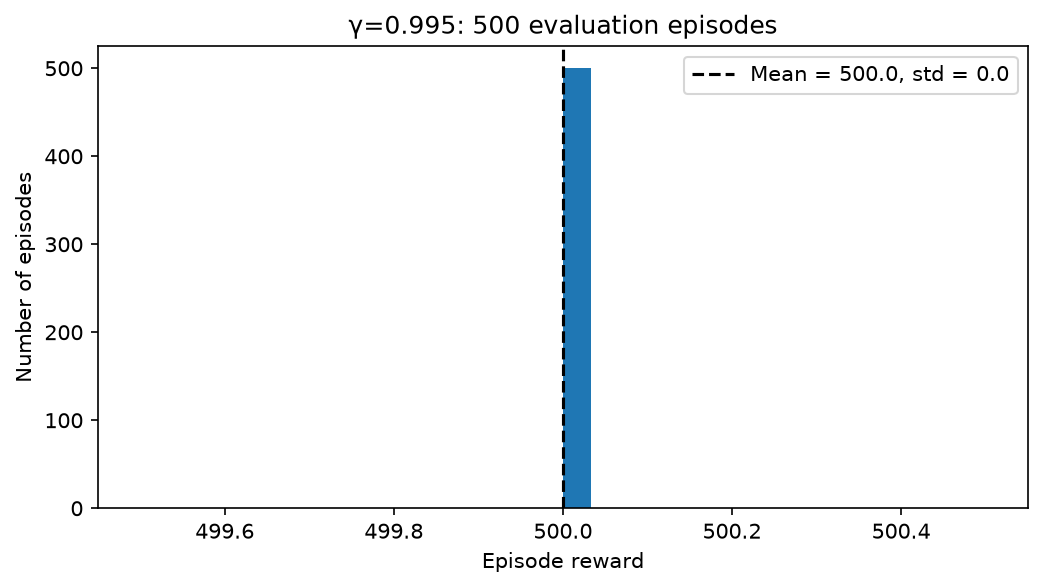
\includegraphics[width=0.32\textwidth]{3a_histogram_gamma.png}\hfill
  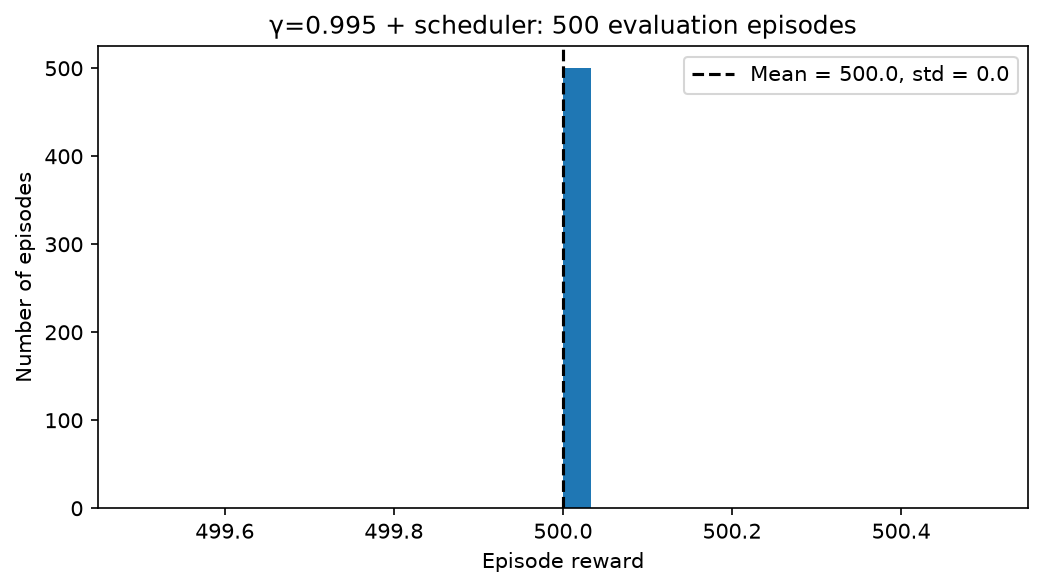
\includegraphics[width=0.32\textwidth]{3a_histogram_scheduler.png}\hfill
  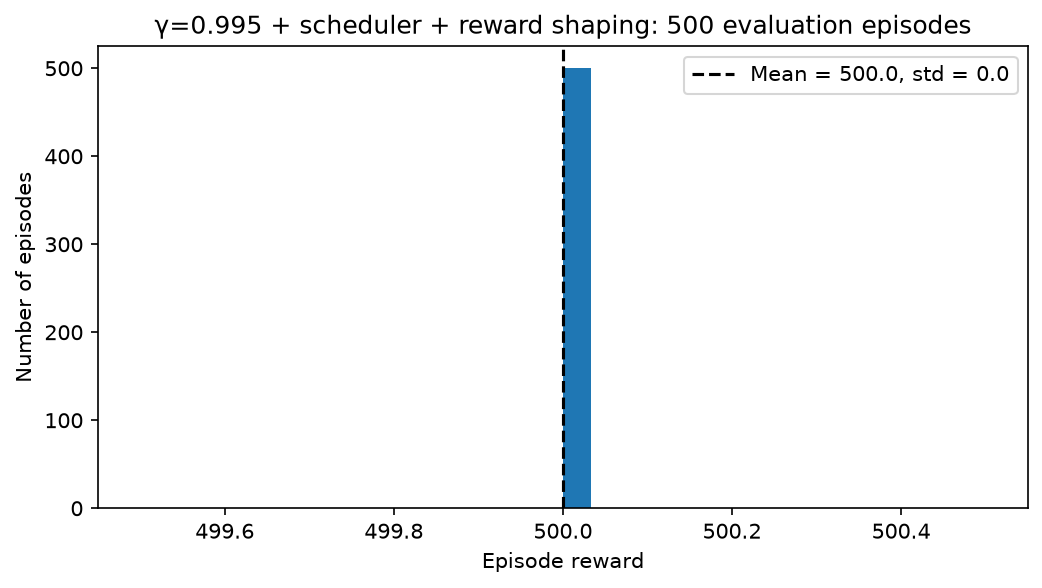
\includegraphics[width=0.32\textwidth]{3a_histogram_shaping.png}
  \caption{Evaluation histograms (500 greedy episodes) of the three variants: $\gamma = 0.995$, + scheduler, + reward shaping.}
  \label{fig:3a-hist-variants}
\end{figure}

\begin{itemize}
  \item \textbf{Bigger $\gamma$:} learning is much faster (more than doubles the mean reward over training), but unstable. The moving average reaches 470 at episode 330 and then collapses to 240.
  \item \textbf{+ Scheduler:} it still dips once while the learning rate is high (to 370 around episode 690). From episode $\sim$780 on, the learning rate is small enough that it stays above 475, whereas $\gamma = 0.995$ alone collapses again at episode 900.
  \item \textbf{+ Reward shaping:} fastest and most stable. From episode 300 on, almost every episode survives 500 steps (81\% of all training episodes).
\end{itemize}

\textbf{For seed 0, all four variants end with a perfect greedy policy.} The hyperparameters therefore improve \textbf{how fast and how reliably} training gets there, which the following experiment and Tests 5--6 confirm.

\subsubsection{Robustness Across Training Seeds}

One training run can be lucky or unlucky, so I trained every variant with 4 more seeds and evaluated each policy greedily on 100 start states (Figure~\ref{fig:3a-seeds}):

\fig{0.7}{3a_seeds.png}{Mean training curve over 5 seeds (band: minimum to maximum).}{fig:3a-seeds}

\begin{center}
\small
\setlength{\tabcolsep}{5pt}
\begin{tabular}{@{}llrrrr@{}}
  \toprule
  \thead[l]{Variant} & \thead[l]{Solved at\\(seeds 0--4)} & \thead[r]{Mean training\\reward} & \thead[r]{Mean of\\last 100} & \thead[r]{Eval.\\mean} & \thead[r]{Eval.\\= 500} \\
  \midrule
  Baseline ($\gamma = 0.95$) & 991, 525, --, --, -- & $192.8 \pm 60.4$ & $292.4 \pm 138.0$ & 362.0 & 3/5 \\
  $\gamma = 0.995$ & 669, 333, 395, --, 662 & $286.3 \pm 78.3$ & $427.6 \pm 127.6$ & 462.2 & 4/5 \\
  + scheduler & 523, 753, 806, 319, 995 & $315.6 \pm 65.3$ & $483.6 \pm 7.4$ & 497.7 & 4/5 \\
  + reward shaping & 341, 327, 659, 494, 604 & $\mathbf{363.3 \pm 48.3}$ & $\mathbf{494.6 \pm 6.8}$ & \textbf{500.0} & \textbf{5/5} \\
  \bottomrule
\end{tabular}

\footnotesize (-- = not solved within 1,000 episodes; ``Eval.\ = 500'': seeds whose greedy evaluation reaches 500 in every episode)
\end{center}

\begin{itemize}
  \item \textbf{Each addition helps on average.} Seed 0 was a lucky run for the baseline: it reaches 475 in only 2 of 5 seeds.
  \item \textbf{The bigger $\gamma$ mostly speeds up learning.} The scheduler mostly makes the end of training reliable: the spread of the last-100 mean drops from $\pm 127.6$ to $\pm 7.4$.
  \item \textbf{Reward shaping is the only variant that solves the task and reaches a perfect greedy policy for every seed.}
\end{itemize}

\subsubsection{Edge Cases}

\begin{center}
\small
\begin{tabularx}{\textwidth}{@{}p{3.6cm}L@{}}
  \toprule
  \textbf{Edge case} & \textbf{Handling} \\
  \midrule
  Invalid arguments & A non-positive number of episodes, $\gamma \notin (0, 1]$ and a scheduler that wraps a different optimizer raise an error (tested). $\gamma = 0$ is excluded because every return would then be the immediate reward of 1, which gives no signal about survival. \\
  Time limit (truncation at 500 steps) & Truncated episodes are treated like terminated ones: the return is cut off, even though the pole is still upright. With $\gamma = 0.95$, this only affects the last $\sim$60 steps (Test 1). The limit also caps the evaluation: no reward can exceed 500, and std = 0 means ``every episode reached the limit'', not a bug. Tested: every reward of 500 is a truncation, every shorter episode a failure. \\
  Saturated evaluation & Since all variants reach 500 in the greedy evaluation, I compare them under harder conditions (Test 5) and over 5 seeds. \\
  Reward shaping must not make failing attractive & The shaped reward is strictly positive ($\geq 0.0016$) on the whole track, so surviving longer always increases the return. With a negative shaped reward (e.g.\ $1 - |x|$), ending the episode early could become optimal. Tested over the whole track. \\
  Shaped vs.\ true reward & The shaped reward is only used to compute the returns. All plots and tables use the environment reward. \\
  Scheduler & Stepped once per episode, over as many steps as there are episodes, so the learning rate ends exactly at 0.001 (tested). It is only stepped if one is used. \\
  Scale of the returns & Returns reach up to $1/(1-\gamma)$: 20 for $\gamma = 0.95$ but 200 for $\gamma = 0.995$. Adam's update does not change when all gradients are scaled by a constant factor, so the same learning rate works for both without retuning. \\
  Start states & $\pm 0.15$ instead of the default $\pm 0.05$, for training and evaluation. A pole angle of 0.15\,rad is already close to the failure angle of 0.21\,rad. Starting at $\pm 0.2$ is tested in Test 5. \\
  Moving average at the start & The first 99 episodes average over fewer episodes. ``Solved at'' only counts full 100-episode windows. \\
  Reproducibility & Seeding PyTorch and the first environment reset makes training reproducible; training twice gives identical rewards (tested). \\
  \bottomrule
\end{tabularx}
\end{center}

\subsubsection{Tests for Validating Correctness}

The tests reuse the trained policies from above, and all of them pass.

\textbf{1. Discounted returns and the credit horizon.} For a constant reward of 1, $G_t = \frac{1 - \gamma^{T-t}}{1 - \gamma}$ must hold, and with $\gamma = 1$, $G_t$ must equal the number of remaining steps. The return computation matches both exactly.

\fig{1.0}{3a_discounting.png}{Discounting: weight of future rewards (left) and the returns of a successful vs.\ a failing episode (right).}{fig:3a-discount}

\begin{center}
\begin{tabular}{@{}lrr@{}}
  \toprule
  $\boldsymbol{\gamma}$ & \textbf{Effective horizon $1/(1-\gamma)$} & $\boldsymbol{\gamma^{100}}$ \\
  \midrule
  0.95 & 20 steps & 0.006 \\
  0.99 & 100 steps & 0.366 \\
  0.995 & 200 steps & 0.606 \\
  \bottomrule
\end{tabular}
\end{center}

With $\gamma = 0.95$, an episode that fails at step 400 has \textbf{the same returns as one that survives all 500 steps for the first $\sim$340 steps} (Figure~\ref{fig:3a-discount}). A slow drift of the cart, which only causes a failure much later, is therefore barely punished. With $\gamma = 0.995$, the later failure lowers the return already at step 0 (173 vs.\ 183). Test 6 checks whether this explains the cart failures of the baseline.

\textbf{2. Control experiments.} Three short trainings (300 episodes, $\gamma = 0.95$) that only differ in the learning signal (Figure~\ref{fig:3a-control}):

\begin{center}
\small
\begin{tabular}{@{}lrrl@{}}
  \toprule
  \thead[l]{Training} & \thead[r]{First 100\\episodes} & \thead[r]{Last 100\\episodes} & \thead[l]{Expected} \\
  \midrule
  Normal & 50.9 & 123.2 & Clearly increases \pass \\
  Learning rate 0 & 20.9 & 21.7 & Flat (the policy never changes) \pass \\
  Negated reward ($-1$ per step) & 15.4 & 10.2 & Learns to fail as fast as possible \pass \\
  \emph{Reference:} random policy & 19.9 & & \\
  \emph{Reference:} always push one way & 9.3 & & \\
  \bottomrule
\end{tabular}
\end{center}

\fig{0.7}{3a_control_experiments.png}{Control experiments: normal training, learning rate 0, and negated reward.}{fig:3a-control}

With the reward flipped, the same code learns the opposite behaviour, getting close to the fastest simple way to fail. This shows that the gradient points in the right direction, and that the improvement in normal training comes from the learning signal, not from chance.

\textbf{3. First 10 steps.} The trained baseline policy, with sampled actions as in training, starting with the pole leaning left ($\theta = -0.138$):

\begin{center}
\small
\setlength{\tabcolsep}{4.5pt}
\begin{tabular}{@{}l*{10}{r}@{}}
  \toprule
  $t$ & 0 & 1 & 2 & 3 & 4 & 5 & 6 & 7 & 8 & 9 \\
  \midrule
  $\theta$ & $-0.138$ & $-0.141$ & $-0.139$ & $-0.132$ & $-0.131$ & $-0.126$ & $-0.116$ & $-0.101$ & $-0.092$ & $-0.078$ \\
  $\dot\theta$ & $-0.15$ & 0.10 & 0.35 & 0.01 & 0.26 & 0.51 & 0.76 & 0.43 & 0.69 & 0.37 \\
  $P(\text{right})$ & 0.03 & 0.05 & 0.14 & 0.03 & 0.08 & 0.24 & \textbf{0.59} & 0.16 & 0.48 & 0.12 \\
  Action & L & L & R & L & L & L & R & L & R & L \\
  \bottomrule
\end{tabular}
\end{center}

\begin{itemize}
  \item \textbf{The policy pushes towards the side the pole leans to} (left) in 9 of 10 steps, so the cart moves back under the pole. It only becomes unsure when the pole already swings back quickly ($\dot\theta = 0.76$ at $t = 6$).
  \item \textbf{As a result, $|\theta|$ shrinks} from 0.138 to 0.071.
  \item The shaped reward stays at 0.568--0.570, the maximum, since the cart stays near the centre.
\end{itemize}

\textbf{4. Does the policy react correctly to the pole?} I vary the pole angle $\theta$ and the angular velocity $\dot\theta$ one at a time, with all other state variables at 0 (Figure~\ref{fig:3a-response}):
\begin{itemize}
  \item For all four policies, $P(\text{right})$ increases monotonically in both, is below 0.5 at the negative end and above 0.5 at the positive end (8 of 8 checks pass). This is the physically correct direction: when the pole leans or falls to the right, the cart must move right.
  \item \textbf{The $\gamma = 0.995$ policy is biased:} it pushes right with probability 0.96 even when the pole is perfectly upright. This explains its drift in Test 6.
\end{itemize}

\fig{1.0}{3a_policy_response.png}{Policy response to the pole angle (left) and the angular velocity (right), all other state variables 0.}{fig:3a-response}

\textbf{5. Harder evaluation.} The greedy evaluation is saturated at 500, so I also evaluate each policy with sampled actions, and with wider start states ($\pm 0.2$; Figure~\ref{fig:3a-robust}):

\begin{center}
\small
\begin{tabular}{@{}lrrr@{}}
  \toprule
  \textbf{Variant} & \textbf{Greedy, $\pm 0.15$} & \textbf{Sampled, $\pm 0.15$} & \textbf{Greedy, $\pm 0.2$} \\
  \midrule
  Baseline ($\gamma = 0.95$) & $500.0 \pm 0.0$ & $482.2 \pm 75.5$ & $500.0 \pm 0.0$ \\
  $\gamma = 0.995$ & $500.0 \pm 0.0$ & $475.0 \pm 104.9$ & $486.7 \pm 78.2$ \\
  + scheduler & $500.0 \pm 0.0$ & $484.6 \pm 62.2$ & $500.0 \pm 0.0$ \\
  + reward shaping & $500.0 \pm 0.0$ & $\mathbf{492.5 \pm 52.8}$ & $500.0 \pm 0.0$ \\
  \bottomrule
\end{tabular}
\end{center}

\fig{0.8}{3a_robustness.png}{Evaluation under harder conditions: sampled actions and wider start states.}{fig:3a-robust}

The reward-shaping policy is the most robust to the noise of sampled actions. The $\gamma = 0.995$ policy, the one with the bias from Test 4, is the only one that fails from wider start states. Overall, the differences between the final policies of seed 0 are small.

\textbf{6. Why do episodes end?} An episode ends when the pole falls ($|\theta| > 12^\circ$), when the cart leaves the track ($|x| > 2.4$), or at the time limit. This checks the explanation from Test 1 (Figures~\ref{fig:3a-ends} and~\ref{fig:3a-cart}):

\begin{center}
\small
\begin{tabularx}{\textwidth}{@{}lLLr@{}}
  \toprule
  \textbf{Variant} & \textbf{Training: cart left / pole fell / 500 steps} & \textbf{Sampled evaluation: cart / pole / 500} & \textbf{Median max $|x|$} \\
  \midrule
  Baseline ($\gamma = 0.95$) & \textbf{564} / 333 / 103 & 0 / 33 / 467 & 0.66 \\
  $\gamma = 0.995$ & 190 / 276 / 534 & 0 / 27 / 473 & 1.25 \\
  + scheduler & 266 / 230 / 504 & 0 / 43 / 457 & 0.68 \\
  + reward shaping & \textbf{14} / 172 / 814 & 0 / 11 / 489 & \textbf{0.26} \\
  \bottomrule
\end{tabularx}

\footnotesize (Median max $|x|$: median over the sampled evaluation episodes of the largest distance of the cart from the centre.)
\end{center}

\fig{1.0}{3a_end_reasons.png}{How training episodes end, per block of 100 episodes.}{fig:3a-ends}

\fig{0.7}{3a_cart_position.png}{Cart position during one greedy episode from the same start state.}{fig:3a-cart}

\begin{itemize}
  \item \textbf{During training, the explanation holds.} With $\gamma = 0.95$, the cart leaves the track in 564 episodes, and this is the most common outcome in 6 of the 10 blocks of 100 episodes. The pole is balanced, but the agent does not see that the cart drifts towards the edge. With $\gamma = 0.995$ there are only 190 such failures, and with reward shaping only 14.
  \item \textbf{The final policies no longer leave the track} (0 cart failures in the evaluation). However, only reward shaping keeps the cart centred (median max $|x| = 0.26$). The $\gamma = 0.995$ policy drifts steadily to $x = -1.26$ within 500 steps, because of the bias from Test 4. It would probably leave the track in a longer episode; only the time limit hides this.
  \item \textbf{Conclusion:} a longer horizon makes it possible to learn to avoid the drift, but does not guarantee it. Only reward shaping rewards staying centred explicitly, and only then is the learned policy centred.
\end{itemize}

\FloatBarrier
\begin{summarybox}{Summary of 3a}
\small
\begin{tabularx}{\linewidth}{@{}lLLLL@{}}
  \toprule
  & \textbf{Baseline ($\gamma = 0.95$)} & \textbf{+ $\gamma = 0.995$} & \textbf{+ scheduler} & \textbf{+ reward shaping} \\
  \midrule
  Solved (5 seeds) & 2/5 & 4/5 & 5/5 & 5/5 \\
  Mean of last 100 episodes (5 seeds) & $292.4 \pm 138.0$ & $427.6 \pm 127.6$ & $483.6 \pm 7.4$ & $494.6 \pm 6.8$ \\
  Greedy evaluation, seed 0 & $500.0 \pm 0.0$ & $500.0 \pm 0.0$ & $500.0 \pm 0.0$ & $500.0 \pm 0.0$ \\
  Main effect & Short horizon: cart drifts off the track & Faster learning & Stable end of training & Fastest, most stable, cart centred \\
  \bottomrule
\end{tabularx}

\medskip
\normalsize
Plain REINFORCE with $\gamma = 0.95$ can solve CartPole, but slowly and unreliably. Each added hyperparameter fixes a specific weakness, and reward shaping has the largest effect.
\end{summarybox}
